%! Author = drakanoy
%! Date = 10.09.2024

% Preamble
\documentclass[12pt]{article}

% Packages
\usepackage[utf8]{inputenc}
\usepackage[T2A]{fontenc}
\usepackage[english, russian]{babel}
\usepackage[a4paper, includefoot, left=1.5cm, right=1.5cm, top=1cm, bottom=1.5cm, headsep=1cm, footskip=1cm]{geometry}
\usepackage{makecell}
\usepackage{amsmath}
\usepackage{graphicx}
\usepackage{enumitem}
\usepackage{svg}
\usepackage{multirow}
\usepackage{hyperref}
\usepackage{mathtools}
\usepackage{amssymb}
\usepackage{textcomp}

% Document
\begin{document}
\begin{large}
\begin{center}
\LARGE \textbf{Домашняя работа}
\par
\LARGE \textbf{Кононов Александр Михайлович}
\par
    \textbf{9.10.2024}
\end{center}
\par Условие:
\par
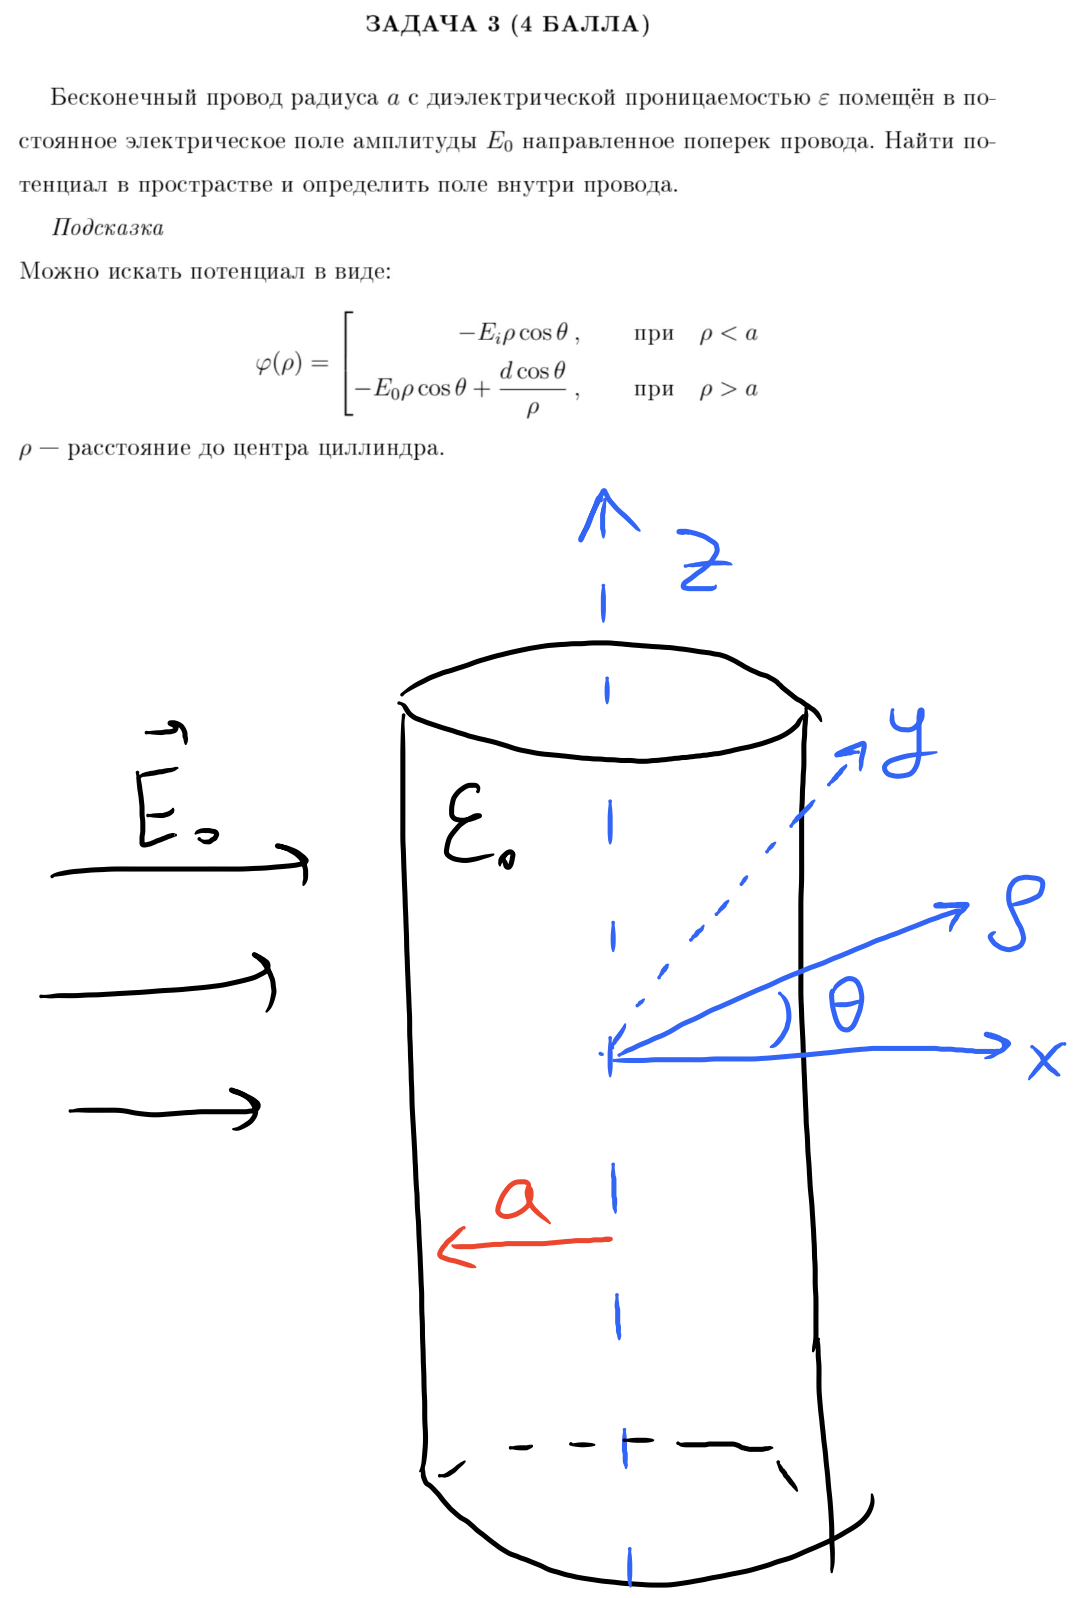
\includegraphics[width=1\textwidth]{photo.png}
%\begin{center}
%\underline{Рисунок 1}:
%\end{center}
\par Решение:
\[
    rot\left( \overrightarrow{B} \right) = \frac{4\pi}{c}\vec{j}
\]
\par Будем искать поле в двух разных полуплоскостях с учетом граничных условий.
\par Для поля в верхней полуплоскости будем искать поле как супер позицию тока заданного и тока в нижний полуплоскости, так как $ rot\left( \overrightarrow{B} \right)$ в верхней полуплоскости может быть равен только заданному току.
\par Для поля в нижней полуплоскости будем искать поле только как результат тока из верхней полуплоскости, так как $ rot\left( \overrightarrow{B} \right)$ в нижней полуплоскости всегда равен $0$ по условию задачи. Там не реальных токов.
\par
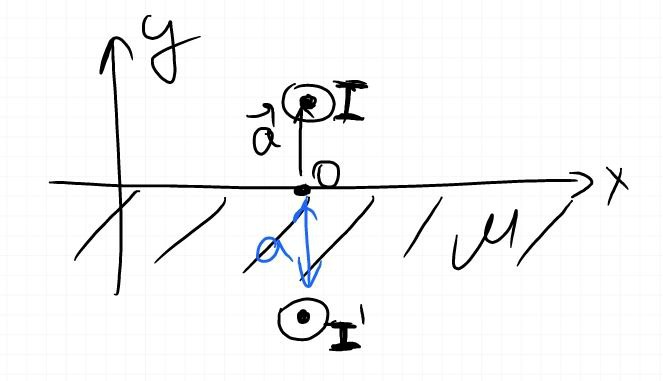
\includegraphics[width=1\textwidth]{photo_1.jpg}
\par
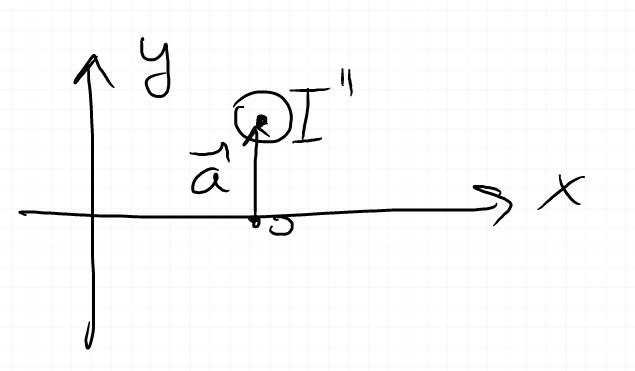
\includegraphics[width=1\textwidth]{photo_2.jpg}
\par
\[
    rot\left( \overrightarrow{B_1} \right) = \frac{4\pi}{c}(\vec{j} + \vec{j}' ) = \frac{4\pi}{c}(\overrightarrow{I} \delta(y-a)\delta(x) + \overrightarrow{I'} \delta(y+a) \delta(x)) \,\,\,\,\, y > 0
\]
\[
    rot\left( \overrightarrow{B_2} \right) = \frac{4\pi}{c}(\vec{j}'' ) = \frac{4\pi}{c}(\overrightarrow{I''} \delta(y-a)\delta(x)) \,\,\,\,\, y < 0
\]
\par Согласно решению о поле бесконечно длинного провода:
\[
    \overrightarrow{B_1} = \frac{2I}{c|\vec{r} - \vec{a}|} \cdot \left[ \vec{e}_z \times \frac{\vec{r} - \vec{a}}{|\vec{r} - \vec{a}|}  \right] + \frac{2I'}{c|\vec{r} + \vec{a}|} \cdot  \left[  \vec{e}_z \times \frac{\vec{r} + \vec{a}}{|\vec{r} + \vec{a}|}  \right]   \,\,\,\,\, y > 0
\]
\[
    \overrightarrow{B_2} = \frac{2I''}{c|\vec{r} - \vec{a}|} \cdot \left[ \vec{e}_z \times \frac{\vec{r} - \vec{a}}{|\vec{r} - \vec{a}|}  \right]   \,\,\,\,\, y < 0
\]
\par Граничные условия:
\[
    B_{n1} = B_{n2} \Rightarrow -I - I' = -I''
\]
\[
    H_{\tau 1} = H_{\tau 2} \Rightarrow I - I' = \frac{I''}{\mu}
\]
\[
    \Rightarrow I' = \frac{\mu - 1}{\mu + 1} I
\]
\[
    I'' = \frac{2 \mu}{\mu + 1} I
\]
\par Ответ:
\[
    \overrightarrow{B_1} = \frac{2I}{c|\vec{r} - \vec{a}|} \cdot \left[ \vec{e}_z \times \frac{\vec{r} - \vec{a}}{|\vec{r} - \vec{a}|}  \right] + \frac{2I}{c|\vec{r} + \vec{a}|} \cdot \frac{\mu - 1}{\mu + 1} \cdot  \left[  \vec{e}_z \times \frac{\vec{r} + \vec{a}}{|\vec{r} + \vec{a}|}  \right]   \,\,\,\,\, y > 0
\]
\[
    \overrightarrow{B_2} = \frac{4I}{c|\vec{r} - \vec{a}|} \cdot \frac{\mu}{\mu + 1}  \cdot \left[ \vec{e}_z \times \frac{\vec{r} - \vec{a}}{|\vec{r} - \vec{a}|}  \right]   \,\,\,\,\, y < 0
\]
\end{large}
\end{document}
